\chapter{Przeprowadzone testy}
\label{ch:tests}
W tym rozdziale omówione zostało przeprowadzenie testów zaimplementowanych algorytmów.

Należy zaznaczyć, że wspomniane w tym rozdziale testy powinny być rozumiane jako eksperymenty przeprowadzenia symulacji planowania tras dla wielu robotów mobilnych, mające na celu zebranie statystycznych danych o przebiegu i rezultatach tych symulacji. Zatem z założenia testy te mogą zakończyć się niepowodzeniem.
Nie należy mylić tego z automatycznymi testami poprawności wykonywanymi podczas powstawania aplikacji w ramach podejścia TDD ({\it Test-Driven Developmnet}), które zostały opisane w jednym z poprzenich rozdziałów (por. \ref{ch:junit-tdd}).

W ramach testów metod planowania tras wykonano pomiary skuteczności oraz wydajności w różnych środowiskach. 
Środowiska te były generowane w sposób losowy, dlatego z obszernych pomiarów zbierano statystyczne wyniki będące wartością średnią mierzonych wskaźników.

Wśród testowanych algorytmów znalazły się:
\begin{itemize}
	\item Algorytm A* bez rozwiązywania kolizji (por. \ref{ch:alg-single-astar}),
	\item LRA* (por. \ref{ch:alg-collision-avoid}),
	\item WHCA*1 bez dynamicznego przydzielania priotytetów (por. \ref{ch:alg-whca}),
	\item WHCA*2 z dynamicznym przydziałem priorytetów (por. \ref{ch:alg-priorities-allocation}),
	\item WHCA*3 z dynamicznym przydziałem priorytetów oraz skalowaniem okna czasowego (por. \ref{ch:alg-priorities-allocation}).
\end{itemize}

Mierzonymi wskaźnikami były:
\begin{itemize}
	\item fakt pomyślnego, bezkolizyjnego doprowadzenia wszystkich robotów do ich celów,
	\item skuteczność rozumiana jako iloraz liczby udanych planowań do liczby wszystkich symulacji,
	\item liczba potrzebnych kroków symulacji (czas wykonywania akcji w rzeczywistym środowisku do momentu doprowadzenia wszystkich robotów do celu),
	\item złożoność obliczeniowa samego planowania (czas wykonywania obliczeń dla wyznaczania tras w ciągu całej symulacji).
\end{itemize}

\section{Automatyczne zarządzanie symulacjami}
Na potrzeby testów, których wyniki zamieszczono w tym rozdziale, przeprowadzono razem $82 800$ automatycznie zarządzanych symulacji. Wykonano to dla różnych metod planowania, w różnych warunkach i na różnych mapach.

Do zarządzania automatycznie wykonywanymi symulacjami wykorzystano bibliotekę {\it jUnit}. Służy ona w standardowym zastosowaniu do wykonywania automatycznych testów jednostkowych sprawdzających poprawność pojedynczych komponentów aplikacji, jednak wykorzystano ją tutaj z powodu możliwości uruchomienia fragmentów aplikacji w innym trybie. Pozwala to na uruchomienie serii symulacji bez wyświetlania graficznego interfejsu użytkownika, które zarządzane są osobnymi fragmentami kodu. Jednocześnie nie powoduje to jakiejkolwiek ingerencji w kod źródłowy głównej aplikacji graficznego sumulatora.
Takie podejście możliwe jest również dzięki zastosowaniu warstwowej architektury MVP (por. \ref{ch:app-mvp}).

Przykładem takiego automatycznego zarządzania symulacjami jest fragment testu utworzonego na potrzeby rozdziału \ref{ch:tests-function-maps-robots}.
W pętli dla kolejnych wartości liczby robotów (od 1 do 30) generowana jest losowa mapę z labiryntem o ustalonej wielkości.
Nastepnie na mapie umieszczane są roboty w losowych polach i przydzielane są im losowe punkty docelowe.
Stanowi to warunki początkowe dla wykonywanej symulacji. Kolejne kroki symulacji wykonywane są sekwencyjnie w sposób ciągły, bez ograniczeń czasowych (bez oczekiwania na kolejne cykle zegarowe, jak w przypadku symulacji z graficznym interfejsem użytkownika).
Następnie odtwarzane są te same warunki początkowe a symulacja wykonywana jest ponownie, tym razem z wykorzystaniem innych metod planowania.
Wszystko to jest powtarzane 1000 razy (dla różnych losowych środowisk) a ze zmierzonych wskaźników obliczana jest wartość średnia.
Liczba sytuacji, w których bezkolizyjne doprowadzenie wszystkich robotów do celu powiodło się, zapisywana jest dla każdej metody planowania osobno.
Wyniki przebiegu symulacji, wyjątkowe zdarzenia oraz obliczone statystyczne wskaźniki wyświetlane są w konsoli a także zapisywane są do pliku dziennika zdarzeń.

Wykonywane symulacje ograniczone są maksymalną liczbą kroków, po przekroczeniu której symulacja jest przerywana i stwierdzane jest niepowodzenie w odnalezieniu bezkolizyjnych tras do celów dla wszystkich robotów.
Zatem sytuacja, w której tylko jeden robot nie znalazł bezkolizyjnej ścieżki do punktu docelowego, jest traktowana tak samo (jako brak rozwiązania), jak gdy żaden z robotów nie dotrze do swojego indywidualnego celu.
Ograniczenie to jest konieczne ze względu na fakt, że w niektórych algorytmach planowania tras (np. LRA*) mogą wystąpić nieskończone cykle zaplanowanych akcji.
Wartość maksymalnej liczby kroków $stepsLimit$ w symulacji została przyjęta arbitralnie na podstawie obserwacji liczby kroków potrzebnych do pomyślnego doprowadzenia robotów do celów przy zmiennej liczbie robotów oraz rozmiarze mapy:

\begin{gather}
 	stepsLimit = (w + h) * r
 	\label{eq:steps-limit} 
\end{gather}
 gdzie:

 $w$ - szerokość mapy (w liczbie pól)

 $h$ - wysokość mapy (w liczbie pól)

 $r$ - liczba robotów na mapie

Warto dodać, że testowane środowiska są bardzo trudnymi warunkami dla metod planowania tras, dlatego skuteczność badanych algorytmów może wydawać się względnie niska, podczas gdy uzycie tych samych metod na innych mapach może skutkować dużo wyższą skutecznością.

\section{Środowiska testowe}
Testy zostały przeprowadzone na czterech typach losowych środowisk, którym dla uproszczenia zapisu nadano nazwy:
\begin{itemize}
	\item {\bf M-15x15-5R} - mapa rozmiaru $15 \times 15$ z wygenerowanym labiryntem, 5 robotów na mapie (por. rys. \ref{fig:test-env-15-15-5}),
	\item {\bf M-15x15-10R} - mapa rozmiaru $15 \times 15$ z wygenerowanym labiryntem, 10 robotów na mapie (por. rys. \ref{fig:test-env-15-15-10}),
	\item {\bf M-35x35-5R} - mapa rozmiaru $35 \times 35$ z wygenerowanym labiryntem, 5 robotów na mapie (por. rys. \ref{fig:test-env-35-35-5}),
	\item {\bf E-15x15-40R} - mapa rozmiaru $15 \times 15$ bez przeszkód, 40 robotów na mapie (por. rys. \ref{fig:test-env-15-15-empty-40}).
\end{itemize}

\begin{figure}
	\centering
	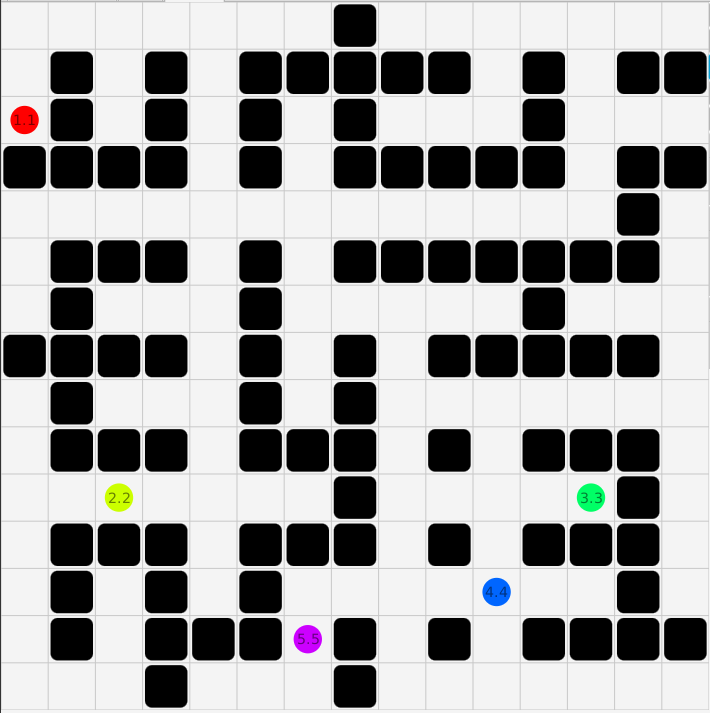
\includegraphics[width=0.6\columnwidth]{img/robopath/tests-15-15-5}
	\caption{Przykładowe środowisko typu M-15x15-5R - mapa $15 \times 15$ z wygenerowanym labiryntem, z 5 robotami w losowych położeniach}
	\label{fig:test-env-15-15-5}
\end{figure}
\begin{figure}
	\centering
	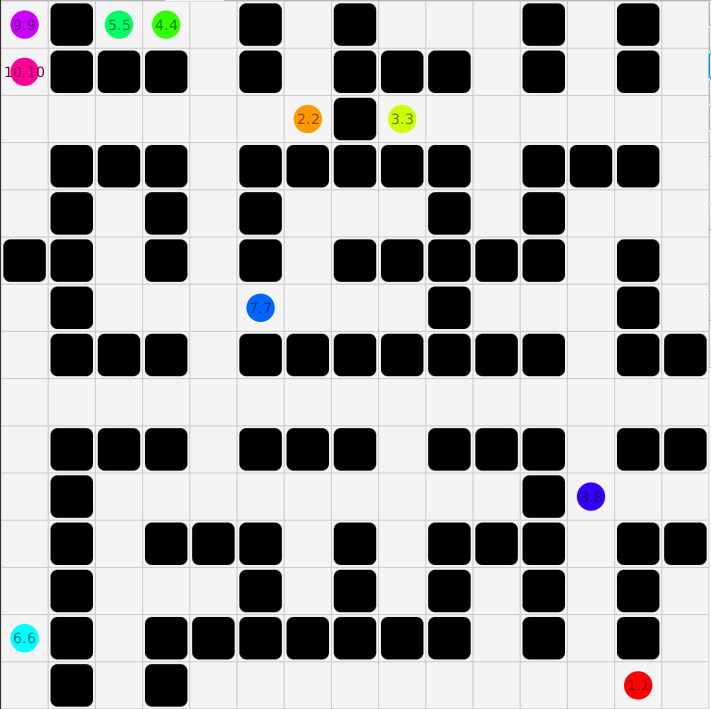
\includegraphics[width=0.6\columnwidth]{img/robopath/tests-15-15-10}
	\caption{Przykładowe środowisko typu M-15x15-10R - mapa $15 \times 15$ z wygenerowanym labiryntem, z 10 robotami w losowych położeniach}
	\label{fig:test-env-15-15-10}
\end{figure}
\begin{figure}
	\centering
	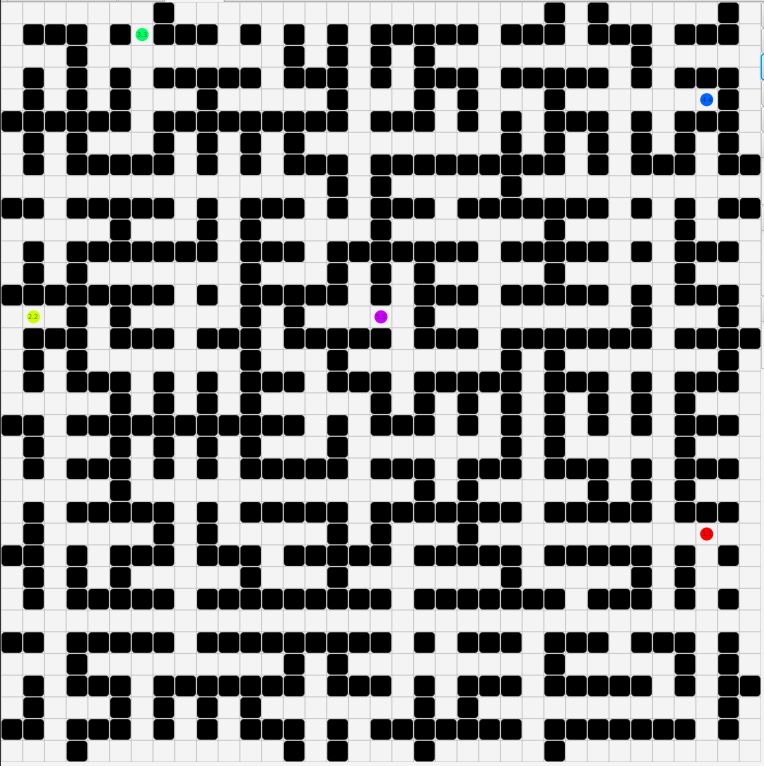
\includegraphics[width=0.6\columnwidth]{img/robopath/tests-35-35-5}
	\caption{Przykładowe środowisko typu M-35x35-5R - mapa $35 \times 35$ z wygenerowanym labiryntem, z 5 robotami w losowych położeniach}
	\label{fig:test-env-35-35-5}
\end{figure}
\begin{figure}
	\centering
	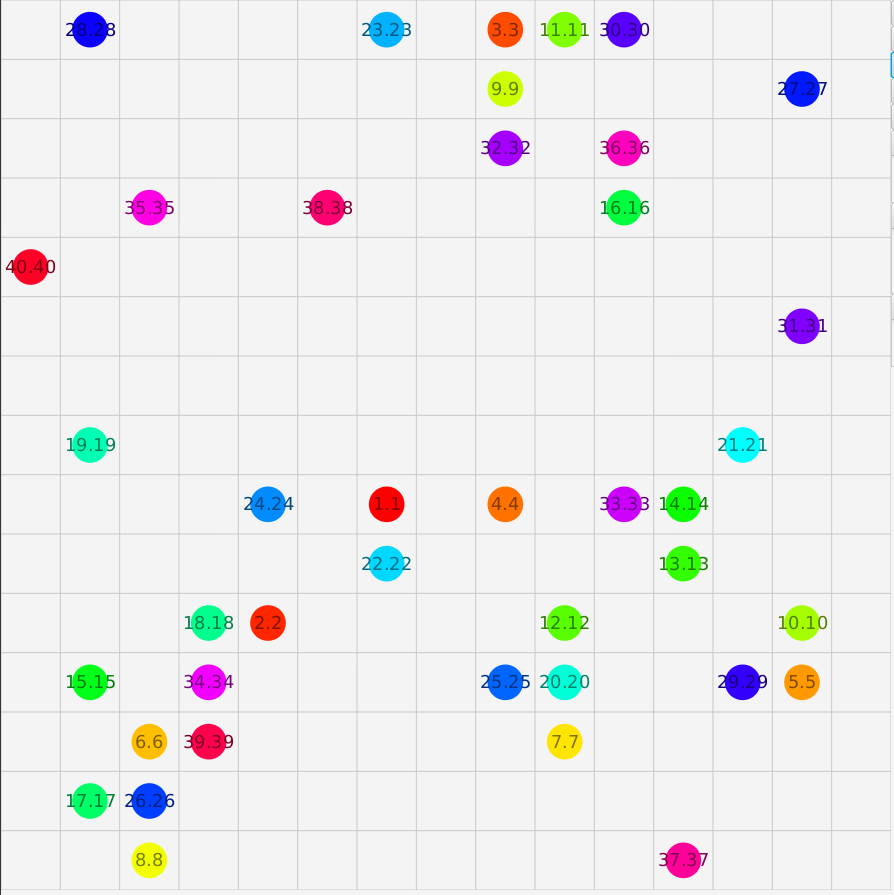
\includegraphics[width=0.6\columnwidth]{img/robopath/tests-15-15-empty-40}
	\caption{Przykładowe środowisko typu E-15x15-40R - mapa $15 \times 15$ bez przeszkód, z 40 robotami w losowych położeniach}
	\label{fig:test-env-15-15-empty-40}
\end{figure}

Dla każdego typu środowiska za każdym razem generowana jest nowa, losowa mapa. Również położenie początkowe i docelowe robotów jest lososwane. Zatem w każdej symulacji wykorzystywane jest inne środowisko, chyba, że porównywane są między sobą różne metody. Wtedy rekonstruowane są te same warunki początkowe, aby przeprowadzić symulację ponownie z wykorzystaniem innej metody planowania.

Każdy z robotów otrzymuje losowe położenie początkowe. Jest to zawsze pole, na którym nie znajduje się przeszkoda, ani nie ma na nim innego robota.
Punkty docelowe także są losowane. Mogą to być pola, na których obecnie znajduje się jakiś robot, natomiast nie może to być punkt docelowy należący do innego robota, gdyż w przeciwnym wypadku uniemożliwiłoby to znalezienie rozwiązania, niezależnie od metody planowania.

\section{Wyniki testów}
\subsection{Częstotliwość występowania potencjalnych kolizji} % 4000
Na początku przeprowadzamy testy częstotliwości występowania potencjalnych kolizji w badanych środowiskach, aby ocenić znaczenie tego problemu.
Dla każdego robota wykonujemy planowanie trasy za pomocą prostego algorytmu A*. Następnie przeprowadzamy symulację ruchu. W momencie wykrycia kolizji robotów zatrzymujemy symulację i zliczamy ilość takich sytuacji. W ten sposób mierzymy, jak często występują kolizję miedzy robotami, jeśli planowanie odbywa się za pomocą algorytmu wyznaczania najkrótszych tras (bez unikania kolizji).
Słuszne jest założenie, że algorytm A* zawsze znajdzie drogę do celu (z pominieciem pozostałych agentów), gdyż w tego typu środowiskach zawsze istnieje połaczenie miedzy dwoma dowolnymi polami na mapie \ref{ch:mazegen}.

W tabeli \ref{tab:test-collision-frequency} przedstawiono wyniki eksperymentów. Skuteczność oznacza w tym przypadku procentową liczbę symulacji, w których ruch wzdłuż zaplanowanych tras odbył się bez żadnych kolizji i wszystkie roboty zostały doprowadzone do celu.
Kolumna "Przeprowadzone symulacje" wyraża liczbę losowo wygenerowanych środowisk określonego typu.

\begin{table}
\caption{Częstotliwosć występowania kolizji w środowiskach zbadana za pomocą skuteczności algorytmu A*} \label{tab:test-collision-frequency} 
\centering
\begin{tabular}{| l | r | r | r |}
\hline
{\bf Typ środowiska} & {\bf Przeprowadzone symulacje} & {\bf Skuteczność} & {\bf Wystąpienie kolizji} \\ \hline
M-15x15-5R  & 1000 & 10\% & 90\% \\ \hline
M-15x15-10R & 1000 & 1\%  & 99\%  \\ \hline
M-35x35-5R  & 1000 & 14\% & 86\% \\ \hline
E-15x15-40R & 1000 & 0\%  & 100\%  \\ \hline
\end{tabular}
\end{table}

W tym teście przeprowadzono razem $4000$ symulacji.

Uzyskane niskie wskaźniki skuteczności potwierdzają, że w tego typu środowiskach, problem występowania kolzji jest bardzo istotny i sam prosty algorytm A* nie wystarcza, aby poradzić sobie z bezkolizyjnym doprowadzeniem wszystkich robotów do celów.

\subsection{Wpływ wielkości okna czasowego} % 400
Zbadano skuteczność metody WHCA*1 (bez dynamicznego przydziału priorytetów) w zależności od wielkości okna czasowego, które to pozostaje stałe w trakcie trwania jednej symulacji.
Dla każdego badanego typu środowiska wylosowano 100 map, dla których powtórzono eksperymenty w tych samych warunkach, ale z różnymi rozmiarami okna czasowego od 1 do 30.
Dla rozmiaru okna równego 1 skuteczność metody zawsze jest zerowa, gdyż zaplanowane dla robotów ścieżki są zawsze długości 1, a pierwszym punktem ścieżki jest zawsze aktualna pozycja robota, przez co roboty pozostają w tym samym miejscu.
Uzyskane wyniki dla każdego środowiska przedstawiono w tabeli \ref{tab:test-whca-window-size} oraz na wykresach \ref{fig:test-whca-window-M-15x15-5R}, \ref{fig:test-whca-window-M-15x15-10R}, \ref{fig:test-whca-window-M-35x35-5R} i \ref{fig:test-whca-window-E-15x15-40R}.

$TODO$ sprawdzić wygląd tabelki
\begin{table}
\caption{Wpływ wielkości okna czasowego na skuteczność metody WHCA*1} \label{tab:test-whca-window-size} 
\centering
\begin{tabular}{| r | r | r | r | r |}
\toprule
{\bf \shortstack{Rozmiar okna\\czasowego}} & \multicolumn{4}{c}{{\bf \shortstack{Skuteczność dla typu środowiska}}} \\
{} &
{\bf \shortstack{M-15x15-5R}} &
{\bf \shortstack{M-15x15-10R}} &
{\bf \shortstack{M-35x35-5R}}} &
{\bf \shortstack{E-15x15-40R}} \\
\midrule
1	& 0\%	& 0\%	& 0\%	& 0\%	\\
2	& 9\%	& 0\%	& 27\%	& 0\%	\\
3	& 11\%	& 0\%	& 30\%	& 0\%	\\
4	& 11\%	& 0\%	& 43\%	& 0\%	\\
5	& 16\%	& 0\%	& 43\%	& 31\%	\\
6	& 21\%	& 0\%	& 48\%	& 65\%	\\
7	& 30\%	& 0\%	& 52\%	& 84\%	\\
8	& 35\%	& 5\%	& 61\%	& 93\%	\\
9	& 42\%	& 5\%	& 61\%	& 96\%	\\
10	& 42\%	& 7\%	& 61\%	& 98\%	\\
11	& 46\%	& 10\%	& 69\%	& 100\%	\\
12	& 53\%	& 12\%	& 74\%	& 100\%	\\
13	& 53\%	& 12\%	& 75\%	& 100\%	\\
14	& 61\%	& 12\%	& 75\%	& 100\%	\\
15	& 61\%	& 20\%	& 82\%	& 100\%	\\
16	& 62\%	& 20\%	& 82\%	& 100\%	\\
17	& 63\%	& 22\%	& 90\%	& 100\%	\\
18	& 64\%	& 23\%	& 90\%	& 100\%	\\
19	& 64\%	& 23\%	& 92\%	& 100\%	\\
20	& 65\%	& 26\%	& 95\%	& 100\%	\\
21	& 65\%	& 26\%	& 100\%	& 100\%	\\
22	& 65\%	& 26\%	& 100\%	& 100\%	\\
23	& 67\%	& 30\%	& 100\%	& 100\%	\\
24	& 67\%	& 33\%	& 100\%	& 100\%	\\
25	& 67\%	& 33\%	& 100\%	& 100\%	\\
26	& 69\%	& 33\%	& 100\%	& 100\%	\\
27	& 69\%	& 33\%	& 100\%	& 100\%	\\
28	& 69\%	& 35\%	& 100\%	& 100\%	\\
29	& 69\%	& 35\%	& 100\%	& 100\%	\\
30	& 69\%	& 35\%	& 100\%	& 100\%	\\
\bottomrule
\end{tabular}
\end{table}

\begin{figure}
	\centering
	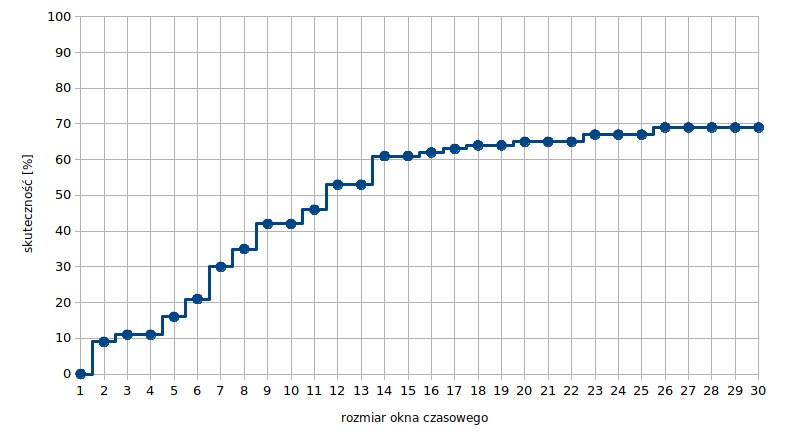
\includegraphics[width=0.8\columnwidth]{img/plots/test-whca-window-M-15x15-5R}
	\caption{Wykres skuteczności metody WHCA* w zależności od rozmiaru okna czasowego dla środowiska typu M-15x15-5R}
	\label{fig:test-whca-window-M-15x15-5R}
\end{figure}
\begin{figure}
	\centering
	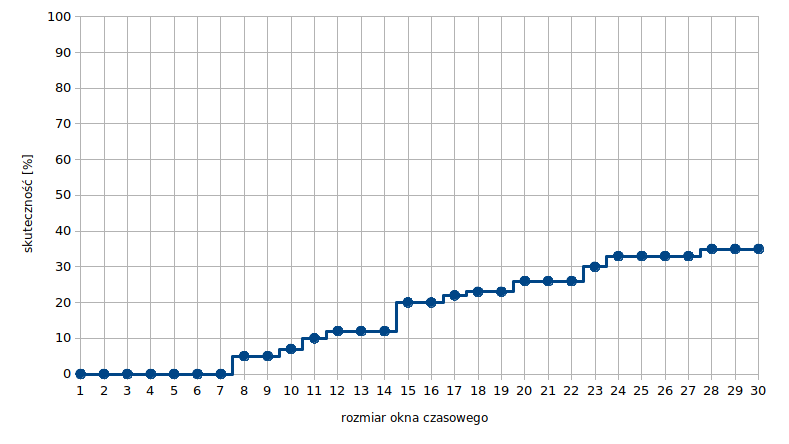
\includegraphics[width=0.8\columnwidth]{img/plots/test-whca-window-M-15x15-10R}
	\caption{Wykres skuteczności metody WHCA* w zależności od rozmiaru okna czasowego dla środowiska typu M-15x15-10R}
	\label{fig:test-whca-window-M-15x15-10R}
\end{figure}
\begin{figure}
	\centering
	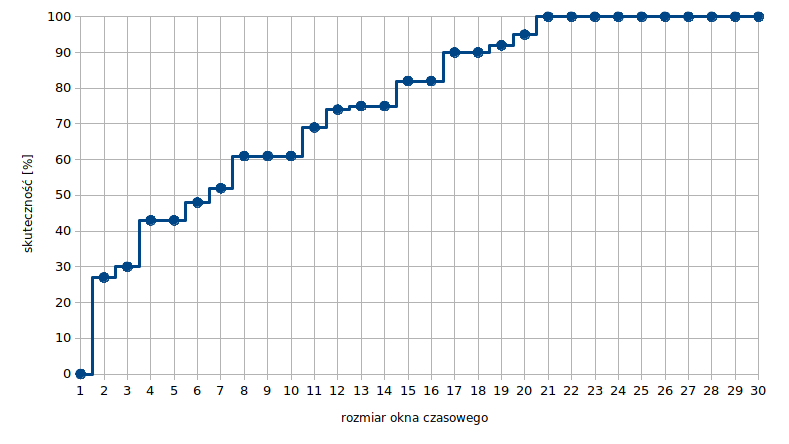
\includegraphics[width=0.8\columnwidth]{img/plots/test-whca-window-M-35x35-5R}
	\caption{Wykres skuteczności metody WHCA* w zależności od rozmiaru okna czasowego dla środowiska typu M-35x35-5R}
	\label{fig:test-whca-window-M-35x35-5R}
\end{figure}
\begin{figure}
	\centering
	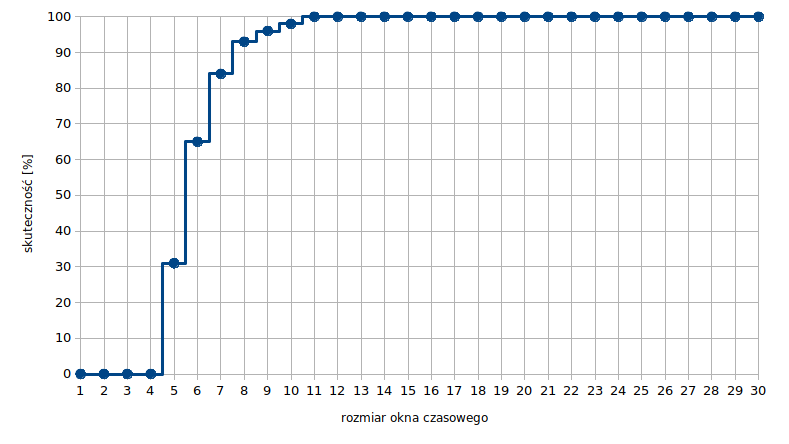
\includegraphics[width=0.8\columnwidth]{img/plots/test-whca-window-E-15x15-40R}
	\caption{Wykres skuteczności metody WHCA* w zależności od rozmiaru okna czasowego dla środowiska typu E-15x15-40R}
	\label{fig:test-whca-window-E-15x15-40R}
\end{figure}

W tym teście przeprowadzono razem $400$ symulacji.

Zgodnie z oczekiwaniami skuteczność metody WHCA*1 rośnie monotonicznie wraz ze wzrostem rozmiaru okna czasowego.

\subsection{Skuteczność LRA* i WHCA*3} %8000
W następnym teście przeprowadzono serie eksperymentów mających na celu porównanie skuteczności metody LRA* oraz WHCA*3 z dynamicznym przydziałem priorytetów.
Mapy generowane były losowo, natomiast dla każdego środowiska symulacja została wykonana dwukrotnie: raz wykonując planowanie tras metodą WHCA* a następnie metodą LRA* po odtworzeniu tych samych warunków początkowych. Dla każdej takiej symulacji zliczano, ile razy obie metody pomyślnie doprowadziły wszystkie roboty do celu, ile razy powiodła się tylko metoda WHCA*3, ile razy tylko metoda LRA*, oraz ile razy żadna z metod nie zakończyła się powodzeniem.
Umożliwiło to porównanie skuteczności metod w dokładnie tych samym warunkach. Wyniki przedstawiono w tabeli \ref{tab:test-lra-whca-effectiveness}.

\begin{table}
\caption{Porównanie skuteczności LRA* i WHCA*3 w tych samych warunkach} \label{tab:test-lra-whca-effectiveness} 
\centering
\begin{tabular}{| l | r | r | r | r | r |}
\hline
{\bf \shortstack{Typ\\środowiska}} &
{\bf \shortstack{Wylosowane\\mapy}} &
{\bf \shortstack{Obie\\udane}} &
{\bf \shortstack{tylko WHCA*\\(dynamiczne\\priorytety)}} &
{\bf \shortstack{tylko\\LRA*}} &
{\bf \shortstack{żadna}} \\ \hline
M-15x15-5R  & 1000 & 230 (23,0\%) & 667 (66,7\%) & 0 (0\%) & 103 (10,3\%) \\ \hline
M-15x15-10R & 1000 & 12  (1,2\%)  & 640 (64,0\%) & 0 (0\%) & 348 (34,8\%) \\ \hline
M-35x35-5R  & 1000 & 513 (51,3\%) & 471 (47,1\%) & 0 (0\%) & 16  (1,6\%)  \\ \hline
E-15x15-40R & 1000 & 823 (82,3\%) & 177 (17,7\%) & 0 (0\%) & 0   (0\%)    \\ \hline
\end{tabular}
\end{table}

W tym teście przeprowadzono razem $8000$ symulacji.

Warto zaznaczyć, że niepowodzenie metody WHCA*3 może wynikać zarówno z ograniczeń metody, jak i z przypadkowego wylosowania układu przeszkód i robotów, który sam w sobie jest niemożliwy do rozwiązania.
Należy także podkreślić, że spośród wszystkich środowisk nie zdarzyło się, aby metoda LRA* dała lepsze rozwiazanie od WHCA*3.
Potwierdza to oczekiwania w stosunku do metody WHCA*3, która jest znacznie bardziej zaawansowana od metody LRA*.

\subsection{WHCA* z dynamicznym przydziałem priorytetów} % 16000
porównanie WHCA*, WHCA* + dynamiczne priorytety, WHCA* + dynamiczne priorytety + dynamiczne okno: skuteczność

poprawność malejącej skuteczności (weryfikowana podczas testów)
testowane na tych samych mapach

\begin{table}
\caption{LRA*, WHCA*, WHCA* + dynamicznymi priorytetami, WHCA* + priorytety + skalowanie okno czasowe} \label{tab:test-lra-whca-whca2-effectiveness} 
\centering
\begin{tabular}{| l | r | r | r | r | r |}
\hline
{\bf \shortstack{Typ\\środowiska}} &
{\bf \shortstack{Wylosowane\\mapy}} &
{\bf \shortstack{Skuteczność\\WHCA*3}} &
{\bf \shortstack{Skuteczność\\WHCA*2}} &
{\bf \shortstack{Skuteczność\\WHCA*1}} &
{\bf \shortstack{Skuteczność\\LRA*}} \\ \hline
M-15x15-5R  & 1000 & 435/500 & 273/500 & 132/500 & 113/500  \\ \hline
M-15x15-10R & 1000 & 272/500 & 244/500 & 17/500  & 1/500    \\ \hline
M-35x35-5R  & 1000 & 493/500 & 349/500 & 200/500 & 264/500  \\ \hline
E-15x15-40R & 1000 & 150/150 & 150/150 & 150/150 & 115/150  \\ \hline
\end{tabular}
\end{table}
$TODO$ zmienić na /1000  i na procenty

W tym teście przeprowadzono razem $16000$ symulacji.

czasem lra był lepszy od whca1 i whca2

\subsection{porównanie parametrów w funkcji rozmiaru mapy i liczby robotów} % 54400
\label{ch:tests-function-maps-robots}
$TODO$ zmergować z 2) - pokrywa sie
1) dla wszystkich, wykres skuteczności 4 algorytmów (serie):
	z labirytntem:
		- w funkcji liczby robotów (15x15) (1-30) * 100 symulacji (3000 sym)
			effect-maze-robots
		- w funkcji rozmiaru mapy (5 robotów) (3x3 - 40x40) * 100 symulacji
			effect-maze-size
	pusta mapa:
		- w funkcji liczby robotów (6x6) (1-30) * 100 symulacji (3000 sym)
			effect-empty-robots
		- w funkcji rozmiaru mapy (5 robotów) (3x3 - 40x40) * 100 symulacji
			effect-empty-size

zachowanie nierówności: WHCA*1 <= WHCA*2 <= WHCA*3
przy wyższych wartościach robotów się zlewają, bo początkowe okno czasowe jest większe
na pustej mapie WHCA*23 dają radę, ale ilość kroków jest duża
zamieszczać też tabelki?

2) dla wszystkich, wykres 4 algorytmów (serie):
	z labirytntem:
		- w funkcji liczby robotów (15x15) (1-30) * 100 symulacji (3000 sym) % 3000 * 4 = 12000
			- średnia liczba kroków (dla udanych)
			- średni czas planowania (dla udanych)
			- skuteczność
				steps-maze-robots
		- w funkcji rozmiaru mapy (5 robotów) (3x3 - 40x40) * 100 symulacji % 3800 * 4 = 15200
			- średnia liczba kroków (dla udanych)
			- średni czas planowania (dla udanych)
			- skuteczność
				steps-maze-mapsize
	pusta mapa:
		- w funkcji liczby robotów (6x6) (1-30) * 100 symulacji (3000 sym) % 3000 * 4 = 12000
			- średnia liczba kroków (dla udanych)
			- średni czas planowania (dla udanych)
			- skuteczność
				steps-empty-robots
		- w funkcji rozmiaru mapy (5 robotów) (3x3 - 40x40) * 100 symulacji % 3800 * 4 = 15200
			- średnia liczba kroków (dla udanych)
			- średni czas planowania (dla udanych)
			- skuteczność
				steps-empty-mapsize

$TODO$ tabelki + wykresy
-- są to tylko przypadki w których udało się LRA, czyli proste układy
pomiar czasu może być obarczony błędami wynikającymi z narzutu JVM i działania Garbage Collectora
wyniki zgodne - zwiększęnie liczby robotów zmniejsza skuteczność, utrudnia znalezienie rozwiązania

\subsection{Metoda pól potencjałowych}
potential field - nawet nie warto testować, raczej jako ciekawostka, nie potrafi doprowadzić do celu nawet jednego robota, screen z minimum lokalnego - studni potencjału
$TODO$

\section{Charakterystyczne przypadki}
$TODO$ screeny ciekawych przypadków

\begin{figure}
	\centering
	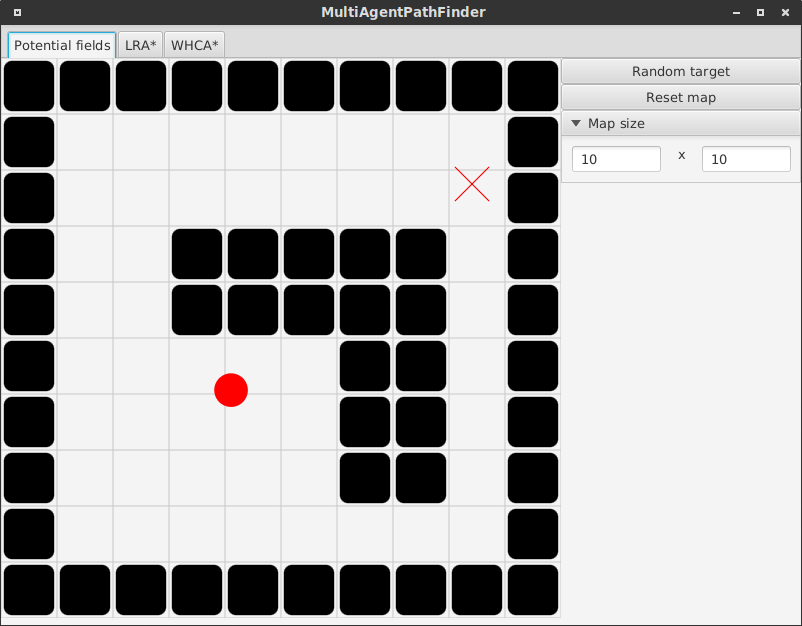
\includegraphics[width=0.8\columnwidth]{img/robopath/field-potential-hole}
	\caption{Robot uwięziony w studni potencjału. Zerowa siła wypadkowa nie pozwala mu dotrzeć do celu.}
	\label{fig:test-field-potential-hole}
\end{figure}

\begin{figure}
	\centering
	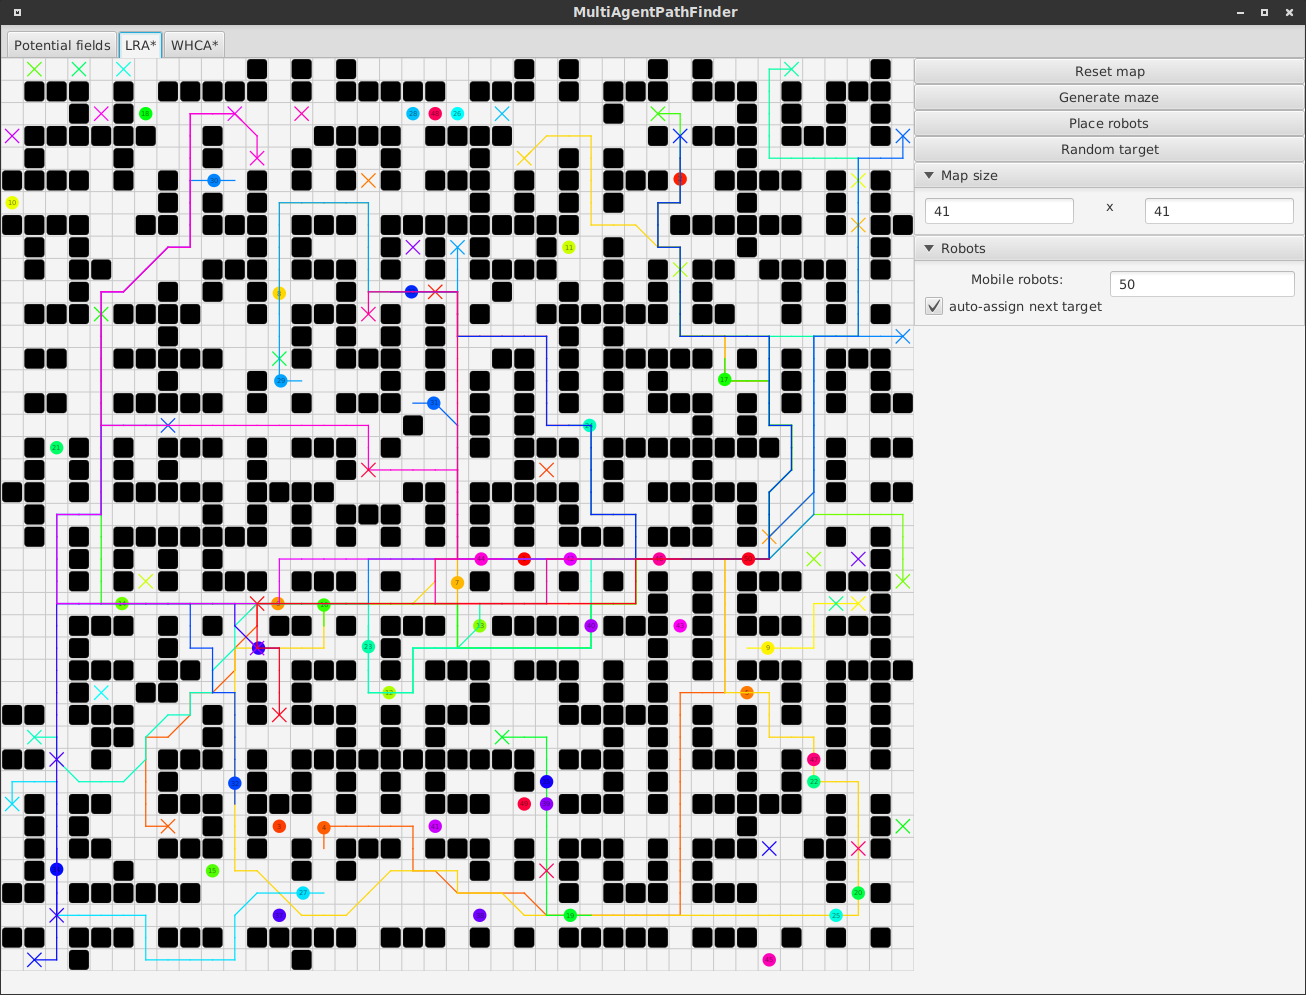
\includegraphics[width=0.8\columnwidth]{img/robopath/lra-bigmap}
	\caption{Metoda LRA*: duża mapa z dużą liczbą robotów}
	\label{fig:test-lra-bigmap}
\end{figure}

% \begin{figure}
% 	\centering
% 	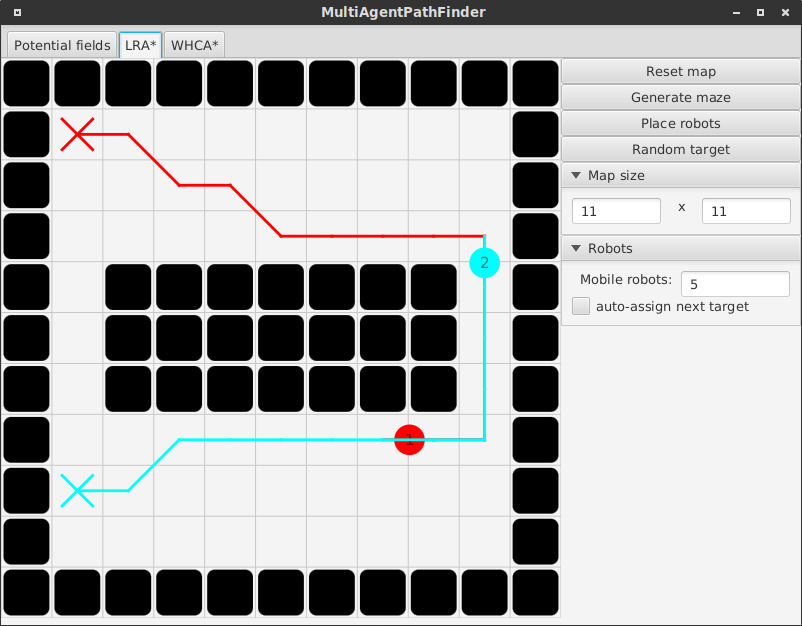
\includegraphics[width=0.8\columnwidth]{img/robopath/lra-cycle}
% 	\caption{Metoda LRA*: 2 roboty w cyklu akcji}
% 	\label{fig:test-lra-cycle}
% \end{figure}

\begin{figure}
	\centering
	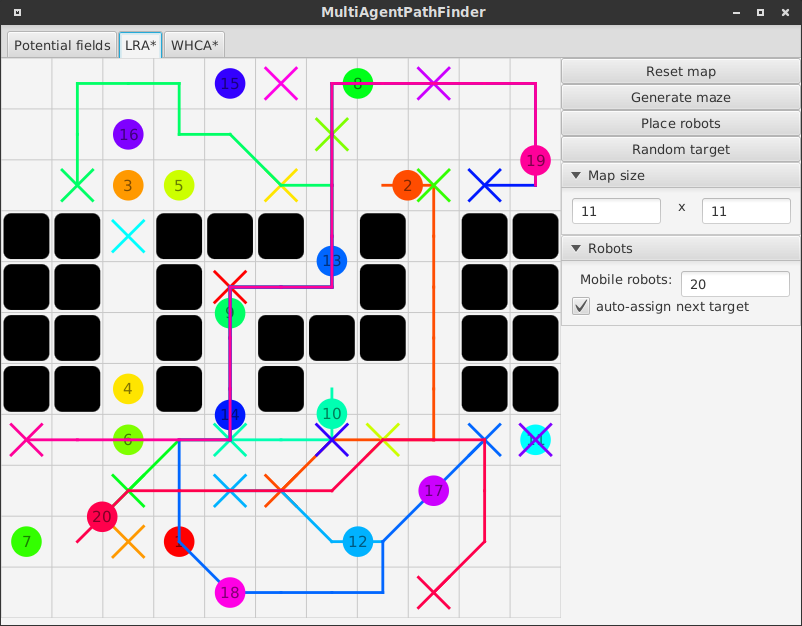
\includegraphics[width=0.8\columnwidth]{img/robopath/lra-lot-robots}
	\caption{Metoda LRA*: dużo robotów, mała mapa}
	\label{fig:test-lra-lot-robots}
\end{figure}

\begin{figure}
	\centering
	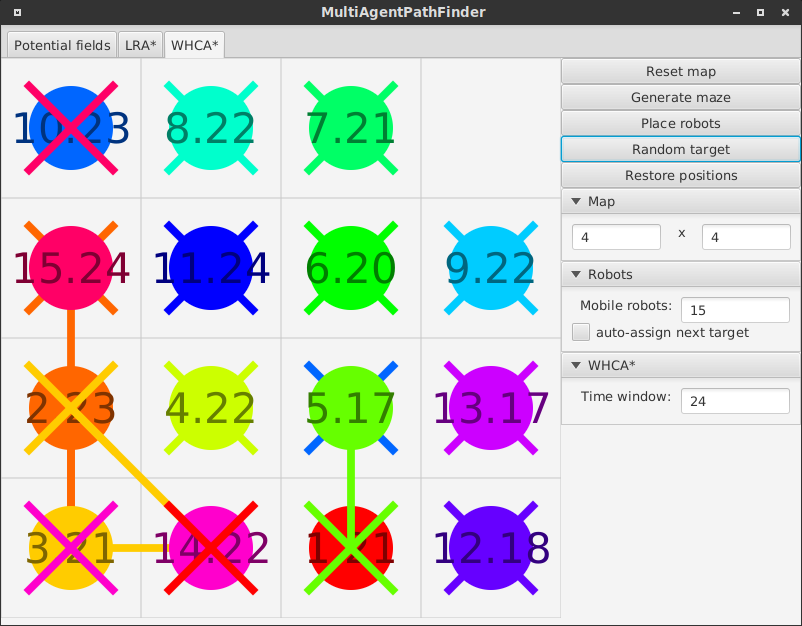
\includegraphics[width=0.8\columnwidth]{img/robopath/puzzle-15}
	\caption{Metoda WHCA*: puzzle 15}
	\label{fig:test-puzzle-15}
\end{figure}

przykład chowania się robotów (przepuszczania się VIPów) - z zaznaczeniem i opisem tras

\section{Dyskusja wyników}
Przeprowadzenie eksperymentów pozwalających wyciągnąć z ich rezultatów niepodważalne wnioski o metodach planowania jest w tym przypadku utrudnione.
Należy pamiętać, że porównanie wyników algorytmów możliwe jest tutaj jedynie w kontekście indywidualnej konfiguracji przeszkód i robotów na mapie.
Nie uzyskujemy ogólnego stwierdzenia, które byłoby prawdziwe dla wszystkich możliwych układów robotów.
Dlatego testy przeprowadzane są w dużej ilości, w losowych środowiskach, następnie posługujemy się statystyką w celu generalizacji uzyskanych rezultatów.

Warto zaznaczyć, że nie dysponujemy kompletną metodą planowania tras, która byłaby w stanie znaleźć zawsze optymalne rozwiązanie lub obiektywnie stwierdzić, że żadne rozwiązanie nie istnieje.
Niestety brak takiego źródła referencyjnego nie pozwala ocenić, czy testowana metoda planowania nie uzyskała rozwiązania z powodu swoich ograniczeń, czy też z powodu tego, że wylosowany układ przeszkód i robotów jest sam w sobie niemożliwy do rozwiązania.
Możliwe jest natomiast porównanie rezultatów różnych metod planowania w tych samych warunkach początkowych, co może jednak dostarczyć pewnych wniosków.


LRA: wyszło całkiem nieźle w przypadku, gdy do celu prowadzi wiele alternatywnych ścieżek i można ominąć wąskie gardło
potwierdzenie oczekiwań (poprawności) - nigdy nie było tak, żeby LRA był lepszy

wolno działa WHCA* przy dużych mapach / oknach czasu / robotach. Dałoby się zoptymalizować (RRA)
autorski WHCA* działa dobrze nawet przy rozwiązywaniu dużych deadlocków, problem z puzzle 15

wada - nie moze się dwóch agentów "cofać". MOże tylko uciekać  z drogi ważniesjzemu


$TODO$ nazwa whca123 w pozostałych rozdziałach
$TODO$ sumaryczna liczba przeprowadzonych symulacji w każdym rozdziale